\documentclass{article}
\usepackage[a4paper, total={6in, 10in}]{geometry}
\usepackage{graphicx}

\title{Project 3 for PSYC 489}
\author{Bingjun Guo (bingjun3)}
\begin{document}
\maketitle
\section*{Part 1}
\subsection*{B.1}
Recordings on each run are in file Part1.txt.\\
Mean hamming distance in each condition: [0.0, 2.0, 3.55, 5.0, 5.8, 6.1].\\
Mean time-to-settle in each condition: [0.0, 12.55, 19.75, 23.1, 24.65, 25.3].\\
The network hasn't failed to settle in each probability condition.
\subsection*{B.2}
Detailed energy recordings are also in Part1.txt. A plot of energy changes on each run is provided below, and we can tell from the plot that energy isn't always decreasing. It increases occasionally. Detailed energy recording is provided in file Part1\_energy.txt.
\begin{figure}[h]
    \centering
    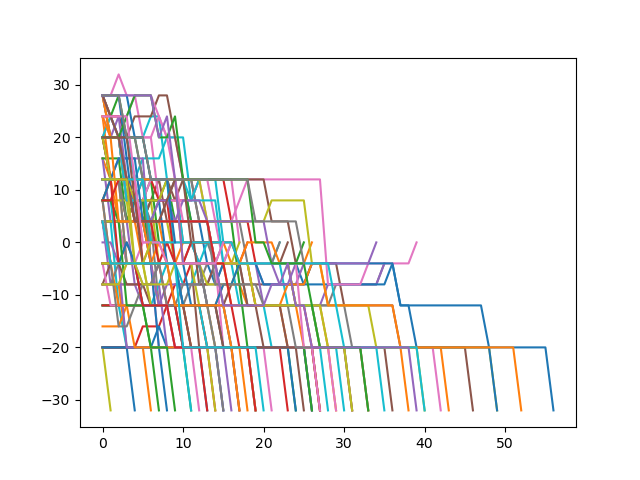
\includegraphics[width=8cm]{Part1energy}
    \caption{Energy on each run in part 1}
\end{figure}
\newpage

\section*{Part 2}
Recordings on each run are in file Part2.txt. Interpretation: It will be harder for the model to settle, that is, both time-to-settle and hamming distances will be larger.\\
Mean hamming distance in each condition: [1.67, 3.07, 4.53, 5.6, 6.47, 6.73].\\
Mean time-to-settle in each condition: [12.2, 19.2, 29.33, 29.47, 31.6, 34.6].\\
The network hasn't failed to settle in each probability condition. Detailed energy recording is in file Part2\_energy.txt.\\
\begin{figure}[h]
    \centering
    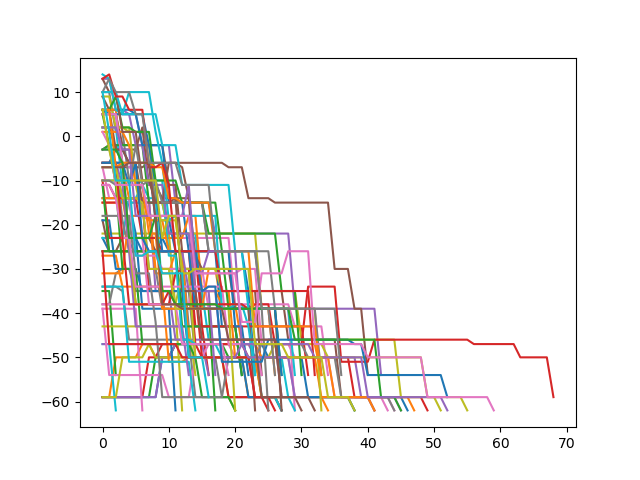
\includegraphics[width=8cm]{Part2energy}
    \caption{Energy on each run in part 2}
\end{figure}\\
It can be observed that mean hamming distances between and time-to-settle are indeed larger, even though the number of training and testing patterns is less. What's more, when the probability is 0, that is, the starting state is exactly the same as a training pattern, the model can fail to settle. It can because that training patterns are random rather than following walsh functions, hence the learning capacity is reduced.\\
In the following runs on two extra patterns, mean hamming distances are 6.6, 5.2 and mean time-to-settle are 37.0, 21.0. Meanwhile, when the probability is 0.2, previous mean values are 4.53 and 29.33. It can be told that hamming distances are larger for the latter two patterns, and time-to-settle are occasionally larger. In Further experiments, it can be observed that they are mostly larger in latter two patterns.
\newpage

\section*{Part 3}


\end{document}
